\documentclass[a4paper, 11pt]{article}
\usepackage[UTF8]{ctex}
\usepackage[cpp,table]{mypackage}
\usepackage{cancel,ulem}
\usepackage{amsmath}
\usepackage{graphicx}
\usepackage{geometry}
\usepackage{listings}
\geometry{scale=0.8}
% \linespread{1.5}
\usepackage[colorlinks,linkcolor=red]{hyperref}

\title{
\normalfont \normalsize
\textsc{School of Data and Computer Science, Sun Yat-sen University} \\ [25pt] %textsc small capital letters
\rule{\textwidth}{0.5pt} \\[0.4cm] % Thin top horizontal rule
\huge  T03 Planning and Uncertainty\\ % The assignment title
\rule{\textwidth}{2pt} \\[0.5cm] % Thick bottom horizontal rule
\author{17341015 陈鸿峥}
\date{\normalsize\today}
}

\begin{document}
\maketitle
\tableofcontents
\newpage

\begin{flushleft}
\textemph{\Large Score: 22/25 + 23/25 + 22/25 + 25/25 = 92}
\end{flushleft}

\section{Q1 - 确定性规划}
\begin{question}\normalfont
Consider a world with pots that may contain water. There is a function $volume(p)$, meaning the volume of pot $p$ in liters. There is a single fluent $Contains(p, w, s)$, meaning that pot $p$ contains $w$ liters of water in situation $s$. There are only two possible actions: $empty(p)$, which can be executed when the pot $p$ is not empty, and which discards all the water contained in $p$, and $transfer(p, p')$, which can be executed when $p \ne p'$, pot $p$ is not empty and pot $p'$ is not full, and which pours as much water as possible without spilling from $p$ to $p'$. To simplify the formalization, we assume that the usual arithmetic constants, functions, and predicates are also available. (You may assume that axioms for these have already been provided or built in.)

Imagine that in the initial situation, we have two pots, a 5-liter one filled with water and an empty 2-liter one. Our goal is to obtain 1 liter of water in the 2-liter pot.

Using the situation calculus, complete the following.
\begin{itemize}
    \item [(a)] Write a sentence describing the initial situation.
    \item [(b)] Write the precondition and effect axioms for the actions.
    \item [(c)] Write a sentence of the form $\exists s.\phi(s)$ that asserts the existence of the final goal situation.
    \item [(d)] Write a ground situation term $\sigma$ such that $\sigma$ denotes the desired goal situation.
\end{itemize}
\end{question}
\begin{answer}
\begin{itemize}
    \item [(a)] 假设两个容器分别为$p_1$和$p_2$,初始情形为
    \[Contains(p_1,5,s_0)\land Contains(p_2,0,s_0)\land volume(p_1)=5\land volume(p_2)=2\]
    \item [(b)] 动作$empty(p)$
    \[\begin{aligned}
        \text{Pre:}\quad & \forall w.(Contains(p,w,s)\land w\ne 0)\\
        \text{Eff:}\quad & Contains(p,0,do(empty(p),s))
    \end{aligned}\]
    动作$transfer(p,p')$
    \[\begin{aligned}
        \text{Pre:}\quad & \forall w,w'.(p\ne p'\bigwedge Contains(p,w,s)\land w\ne 0\bigwedge Contains(p',w',s)\land w'\ne volume(p'))\\
        \text{Eff:}\quad & \quad (w > volume(p')-w'\\
        &\quad \land Contains(p,w-volume(p')+w',do(transfer(p,p'),s))\\
        &\quad \land Contains(p',volume(p'),do(transfer(p,p'),s)))\\
        &\bigvee (w <= volume(p') -w'\\
        &\quad \land Contains(p,0,do(transfer(p,p'),s))\\
        &\quad \land Contains(p',volume(p')-w'+w,do(transfer(p,p'),s)))
    \end{aligned}\]
    因$transfer(p,p')\equiv \text{Pre}\to \text{Eff}$,故$\text{Eff}$的量词$\forall w,w'$在此省略。
    \item [(c)] 目标情形如下
    \[\exists s.Contains(p_2,1,s)\]
    \item [(d)] 目标情形可以表示如下
    \[\sigma=do(transfer(p_1,p_2),do(empty(p_2),do(transfer(p_1,p_2),do(empty(p_2),do(transfer(p_1,p_2),s_0)))))\]
    两个容器的水量变化如下表所示
    \begin{center}
    \begin{tabular}{|c|c|c|}\hline
        action & $p_1$ & $p_2$\\\hline
        $transfer(p_1,p_2)$ & 3 & 2 \\\hline
        $empty(p_2)$ & 3 & 0 \\\hline
        $transfer(p_1,p_2)$ & 1 & 2 \\\hline
        $empty(p_2)$ & 1 & 0 \\\hline
        $transfer(p_1,p_2)$ & 0 & 1 \\\hline
    \end{tabular}
    \end{center}
\end{itemize}
\end{answer}
\begin{flushleft}
\textemph{
Score: 22/25
\begin{itemize}
\item (b) transfer的effect错,最后一句应该是
\[Contains(p',w'+w,do(transfer(p,p'),s)\]
\end{itemize}
}
\end{flushleft}

\newpage
\section{Q2 - STRIPS}
\begin{question}\normalfont
Consider the following blocks world planning problem.
There are a collection of blocks: a block can be on the table, or on top of another block.
There are three predicates:
$clear(x)$: there is no block on top of block $x$;
$on(x, y)$: block $x$ is on top of block $y$; and
$onTable(x)$: block $x$ is on the table.
There are three actions:
$move(x, y, z)$: move block $x$ from block $y$ onto block $z$, provided $x$ is on $y$, both $x$ and $z$ are clear;
$moveFromTable(x, y)$: move block $x$ from the table onto block $y$, provided $x$ is on the table, both $x$ and $y$ are clear; and
$moveToTable(x, y)$: move block $x$ from block $y$ onto the table, provided $x$ is on $y$, and $x$ is clear.

The initial state is
\begin{tabular}{|c|}\hline
a\\\hline b\\\hline c\\\hline
\end{tabular}
\qquad The goal state is
\begin{tabular}{|c|}\hline
a\\\hline b\\\hline
\end{tabular}
\quad
\begin{tabular}{|c|}\hline
c\\\hline
\end{tabular}
\begin{itemize}
    \item [(a)] Write the STRIPS representation of the actions, the initial KB, and the goal.
    \item [(b)] Use reachability analysis to compute the heuristic value for the initial state. Draw the state and action layers. For each call of CountActions, indicate the values of G, GP, GN, and A.
\end{itemize}
\end{question}
\begin{answer}
\begin{itemize}
    \item [(a)] 初始数据库:
    \[KB=\{clear(a),on(a,b),on(b,c),onTable(c)\}\]
    动作$move(x,y,z)$:
    \[\begin{aligned}
        Pre:&\{on(x,y),clear(x),clear(z)\}\\
        Add:&\{on(x,z),clear(y)\}\\
        Del:&\{on(x,y),clear(z)\}
    \end{aligned}\]
    动作$moveFromTable(x,y)$:
    \[\begin{aligned}
        Pre:&\{onTable(x),clear(x),clear(y)\}\\
        Add:&\{on(x,y)\}\\
        Del:&\{onTable(x),clear(y)\}
    \end{aligned}\]
    动作$moveToTable(x,y)$:
    \[\begin{aligned}
        Pre:&\{on(x,y),clear(x)\}\\
        Add:&\{clear(y),onTable(x)\}\\
        Del:&\{on(x,y)\}
    \end{aligned}\]
    目标:
    \[Goal=\{clear(a),clear(c),on(a,b),onTable(b),onTable(c)\}\]
    \item [(b)] 如下所示,$Goal\subset S_2$
    \[\begin{aligned}
        S_0 :&\{clear(a),on(a,b),on(b,c),onTable(c)\}\\
        A_0 :&\{\textcolor{red}{moveToTable(a,b)}\}\\
        S_1 :&\{clear(a),on(a,b),on(b,c),onTable(c),\textcolor{red}{clear(b),onTable(a)}\}\\
        A_1 :&\{\textcolor{orange}{move(a,b,a)},\textcolor{blue}{move(b,c,a)},\textcolor{purple}{moveToTable(b,c)},\\
         & \textcolor{green}{moveFromTable(a,a)},\textcolor{cyan}{moveFromTable(a,b)}\}\\
        S_2 :&\{\underline{clear(a),\textcolor{cyan}{on(a,b)}},on(b,c),\underline{onTable(c)},clear(b),onTable(a),\\
         & \textcolor{orange}{on(a,a)},\textcolor{blue}{on(b,a),\underline{clear(c)}},\textcolor{purple}{\underline{onTable(b)}}\}
    \end{aligned}\]
    \begin{figure}[H]
        \centering
        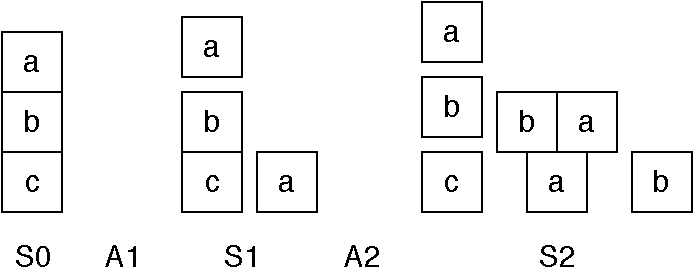
\includegraphics[width=0.6\linewidth]{fig/T03-Q2.pdf}
    \end{figure}
    \textemph{注意这里图中的动作层标号有误}\\
    由$S_2$可得
    \[\begin{aligned}
        G&=\{clear(a),clear(c),on(a,b),onTable(b),onTable(c)\}\\
        G_P&=\{clear(a),on(a,b),onTable(c)\}\\
        G_N&=\{\textcolor{purple}{clear(c),onTable(b)}\}\\
        A&=\{[\underline{on(b,c),clear(b)}]moveToTable(b,c)[\textcolor{purple}{clear(c),onTable(b)}]\}\\
        G_1&=G_P\cup Pre(A)=\{clear(a),on(a,b),onTable(c),\underline{on(b,c),clear(b)}\}
    \end{aligned}\]
    \[CountActions(G,S_2)=1+CountActions(G_1,S_1)\]
    由$S_1$可得
    \[\begin{aligned}
        G_P&=\{clear(a),on(a,b),onTable(c),on(b,c)\}\\
        G_N&=\{\textcolor{red}{clear(b)}\}\\
        A&=\{[\underline{on(a,b),clear(a)}]moveToTable(a,b)[\textcolor{red}{clear(b)},onTable(a)]\}\\
        G_2&=G_P\cup Pre(A)=\{\underline{clear(a),on(a,b)},onTable(c),on(b,c)\}
    \end{aligned}\]
    \[CountActions(G_1,S_1)=1+CountActions(G_2,S_0)\]
    进而得到
    \[CountActions(G,S_2)=1+1+0=2\]
\end{itemize}
\end{answer}
\begin{flushleft}
\textemph{
Score: 23/25
\begin{itemize}
\item (b) $A1$层动作不全,应该有一下这些
\[\begin{aligned}
&move(a,a,a),move(a,a,b),move(a,b,b),move(b,c,a),move(b,c,b),\\
&moveFromTable(a,a),moveFromTable(a,b),\\
&moveToTable(a,a),moveToTable(b,c)
\end{aligned}\]
\end{itemize}
}
\end{flushleft}

\newpage
\section{Q3 - 贝叶斯网络}
\begin{question}\normalfont
Consider the following example: Metastatic cancer is a possible cause of a brain tumor and is also an explanation for an increased total serum calcium. In turn, either of these could cause a patient to fall into an occasional coma. Severe headache could also be explained by a brain tumor.
\begin{itemize}
    \item [(a)] Represent these causal links in a belief network. Let $a$ stand for metastatic cancer, $b$ for increased total serum calcium, $c$ for brain tumor, $d$ for occasional coma, and $e$ for severe headaches.
    \item [(b)] Give an example of an independence assumption that is implicit in this network.
    \item [(c)] Suppose the following probabilities are given:
\[\begin{array}{rllrll}
{P(a)} & {=} & {0.2} & {} \\
{P(b \mid a)} & {=} & {0.8} & {P(b \mid \neg a)} & {=} & {0.2} \\
{P(c \mid a)} & {=} & {0.2} & {P(c \mid \neg a)} & {=} & {0.05} \\
{P(e \mid c)} & {=} & {0.8} & {P(e \mid \neg c)} & {=} & {0.6} \\
{P(d \mid b, c)} & {=} & {0.8} & {P(d \mid \neg b, c)} & {=} & {0.8} \\
{P(d \mid b, \neg c)} & {=} & {0.8} & {P(d \mid \neg b, \neg c)} & {=} & {0.05}
\end{array}\]
    and assume that it is also given that some patient is suffering from severe headaches but has not fallen into a coma. Calculate joint probabilities for the eight remaining possibilities (that is, according to whether $a$, $b$, and $c$ are true or false).
    \item [(d)] According to the numbers given, the a priori probability that the patient has metastatic cancer is $0.2$. Given that the patient is suffering from severe headaches but has not fallen into a coma, are we now more or less inclined to believe that the patient has cancer? Explain.
\end{itemize}
\end{question}
\begin{answer}
\begin{itemize}
    \item [(a)] 贝叶斯网络如下图所示
\begin{figure}[H]
\centering
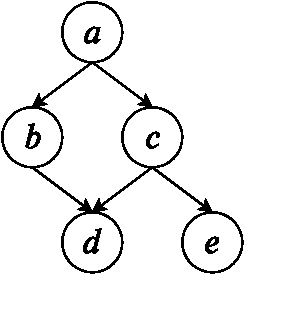
\includegraphics[width=0.2\linewidth]{fig/T03-Q3-A.pdf}
\end{figure}
    \item [(b)] 给定$b$和$c$的前提下,$d$与$a$和$e$独立,即
    \[P(d\mid a,b,c,e)=P(d\mid b,c)\]
    \item [(c)] 题目要求$P(A,B,C,\lnot d,e)$的联合概率,详细的代入过程已忽略,只给出核心步骤及最终结果。
    \[\begin{aligned}
        &P(a,b,c,\lnot d,e) &=& P(a) P(b\mid a) P(c\mid a) P(\lnot d\mid b,c) P(e\mid c) &= 0.00512\\
        &P(a,b,\lnot c,\lnot d,e) &=& P(a) P(b\mid a) P(\lnot c\mid a) P(\lnot d\mid b,\lnot c) P(e\mid \lnot c) &= 0.01536\\
        &P(a,\lnot b,c,\lnot d,e) &=& P(a) P(\lnot b\mid a) P(c\mid a) P(\lnot d\mid \lnot b,c) P(e\mid c) &= 0.00128\\
        &P(a,\lnot b,\lnot c,\lnot d,e) &=& P(a) P(\lnot b\mid a) P(\lnot c\mid a) P(\lnot d\mid \lnot b,\lnot c) P(e\mid \lnot c) &= 0.01824\\
        &P(\lnot a,b,c,\lnot d,e) &=& P(\lnot a) P(b\mid \lnot a) P(c\mid \lnot a) P(\lnot d\mid b,c) P(e\mid c) &= 0.00128\\
        &P(\lnot a,b,\lnot c,\lnot d,e) &=& P(\lnot a) P(b\mid \lnot a) P(\lnot c\mid \lnot a) P(\lnot d\mid b,\lnot c) P(e\mid \lnot c) &= 0.01824\\
        &P(\lnot a,\lnot b,c,\lnot d,e) &=& P(\lnot a) P(\lnot b\mid \lnot a) P(c\mid \lnot a) P(\lnot d\mid \lnot b,c) P(e\mid c) &= 0.00512\\
        &P(\lnot a,\lnot b,\lnot c,\lnot d,e) &=& P(\lnot a) P(\lnot b\mid \lnot a) P(\lnot c\mid \lnot a) P(\lnot d\mid \lnot b,\lnot c) P(e\mid \lnot c) &= 0.34656
    \end{aligned}\]
    \item [(d)] 即计算$P(a\mid\lnot d,e)$,由贝叶斯公式
    \[P(a\mid\lnot d,e)=\frac{P(a,\lnot d,e)}{P(\lnot d,e)}\]
    则由(c),
    \[\begin{aligned}
        P(a,\lnot d,e)&=\sum_{b,c} P(a,b,c,\lnot d,e)=0.04\\
        P(\lnot d,e)&=\sum_{a,b,c} P(a,b,c,\lnot d,e)=0.4112
    \end{aligned}\]
    进而,$P(a\mid\lnot d,e)=0.04/0.4112=0.097276<P(a)=0.2$,故病人有癌症的概率降低了。
\end{itemize}
\end{answer}
\begin{flushleft}
\textemph{
Score: 22/25
\begin{itemize}
\item 题目要求$P(A,B,C\mid\lnot d,e)$,(c)题都要除以$P(\lnot d,e)$
\end{itemize}
}
\end{flushleft}

\newpage
\section{Q4 - 变量消除算法}
\begin{question}\normalfont
Consider the following belief network:

\begin{minipage}{0.5\linewidth}
\begin{figure}[H]
\centering
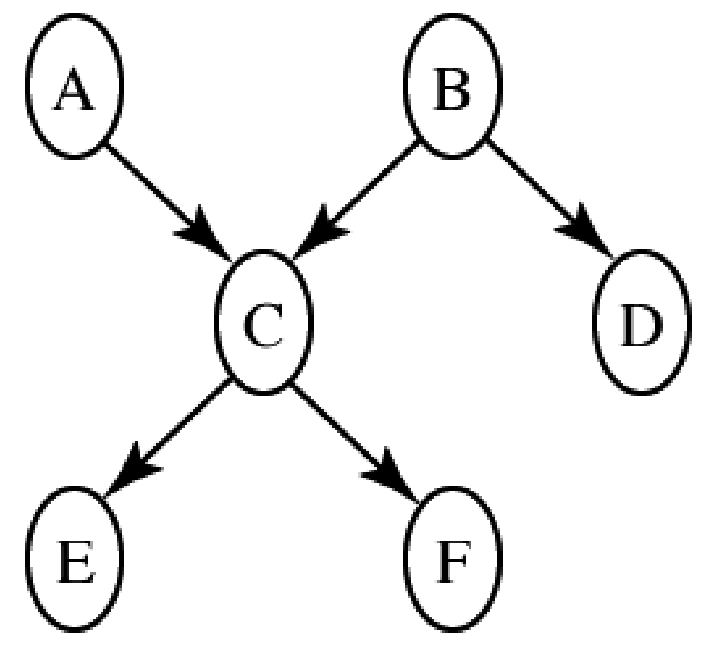
\includegraphics[width=0.6\linewidth]{fig/Q4.png}
\end{figure}
\end{minipage}
\begin{minipage}{0.5\linewidth}
\[\begin{aligned}
P(a) &=0.9 \quad P(d \mid b) &=0.1 \\
P(b) &=0.2 \quad P(d \mid \neg b)&=0.8 \\
P(c \mid a, b) &=0.1 \quad P(e \mid c)&=0.7 \\
P(c \mid a,\neg b) &=0.8 \quad P(e \mid \neg c)&=0.2 \\
P(c \mid \neg a, b) &=0.7 \quad P(f \mid c)&= 0.2 \\
P(c \mid \neg a, \neg b) &=0.4 \quad P(f \mid \neg c)&= 0.9
\end{aligned}\]
\end{minipage}
\begin{itemize}
    \item [(a)] Compute $P(e)$ using VE. You should first prune irrelevant variables. Show the factors that are created for a given elimination ordering.
    \item [(b)] Suppose you want to compute $P(e\mid\lnot f)$ using VE. How much of the previous computation can be reused? Show the factors that are different from those in part (a).
\end{itemize}
\end{question}
\begin{answer}
\begin{itemize}
    \item [(a)] 相关变量有$a,b,c,e$,无关变量为$d,f$,记$A,B,C,E$的CPT分别为$f_1(A)$,$f_2(B)$,$f_3(A,B,C)$,$f_4(C,E)$,按照$A,B,C$的顺序消除。
    \[f_5(B,C)=\sum_a f_1(a)f_3(a,B,C)=\text{\begin{tabular}{|c|c|c|}\hline
        $c$ & $b$ & $0.16$\\\hline
        $c$ & $\lnot b$ & $0.76$\\\hline
        $\lnot c$ & $b$ & $0.04$\\\hline
        $\lnot c$ & $\lnot b$ & $0.04$\\\hline
    \end{tabular}}\]
    \[f_6(C)=\sum_b f_2(b)f_5(b,C)=\text{\begin{tabular}{|c|c|}\hline
        $c$ & $0.64$\\\hline
        $\lnot c$ & $0.36$\\\hline
    \end{tabular}}\]
    \[f_7(E)=\sum_c f_6(c)f_4(c,E)=\text{\begin{tabular}{|c|c|}\hline
        $e$ & $0.52$\\\hline
        $\lnot e$ & $0.48$\\\hline
    \end{tabular}}\]
    故$P(e)=0.52$。
    \item [(b)] 相关变量为$a,b,c,e,f$,无关变量为$d$。
    $f_1(A),f_2(B),f_3(A,B,C),f_5(B,C)$和$f_6(C)$都可以复用,其他不同的因子为$f_9(C)$,$f_{10}(C,E)$,$f_{11}(E)$,具体步骤如下:
    \begin{enumerate}
        \item 限制$F$为$\lnot f$,用
        \[f_9(C)=f_8(C,\lnot f)=\text{\begin{tabular}{|c|c|}\hline
            $c$ & $0.8$\\\hline
            $\lnot c$ & $0.1$\\\hline
        \end{tabular}}\]
        代替$f_8(C,F)$
        \item 消除$A,B$依次得到$f_5(B,C)$和$f_6(C)$(复用(a)的结果)
        \item 消除$C$,所有含$C$的因子$f_6(C),f_9(C),f_4(C,E)$相乘有
        \[f_{10}(C,E)=f_4(C,E)\times f_6(C)\times f_9(C)=\text{\begin{tabular}{|c|c|c|}\hline
            $c$ & $e$ & $0.3584$\\\hline
            $c$ & $\lnot e$ & $0.1536$\\\hline
            $\lnot c$ & $e$ & $0.072$\\\hline
            $\lnot c$ & $\lnot e$ & $0.0288$\\\hline
        \end{tabular}}\]
        \item 最后消除$C$,得到
        \[f_{11}(E)=\sum_c f_{10}(c,E)=\text{\begin{tabular}{|c|c|}\hline
            $e$ & $0.3656$\\\hline
            $\lnot e$ & $0.1824$\\\hline
        \end{tabular}}\]
        \item 归一化得到
        \[P(e\mid\lnot f)=0.3656/(0.3656+0.1824)=0.66715\]
    \end{enumerate}
\end{itemize}
\end{answer}
\begin{flushleft}
\textemph{
Score: 25/25
}
\end{flushleft}

\end{document}